\clearpage\section*{Route counting: Overloaded active layers (\%)}
\begin{center}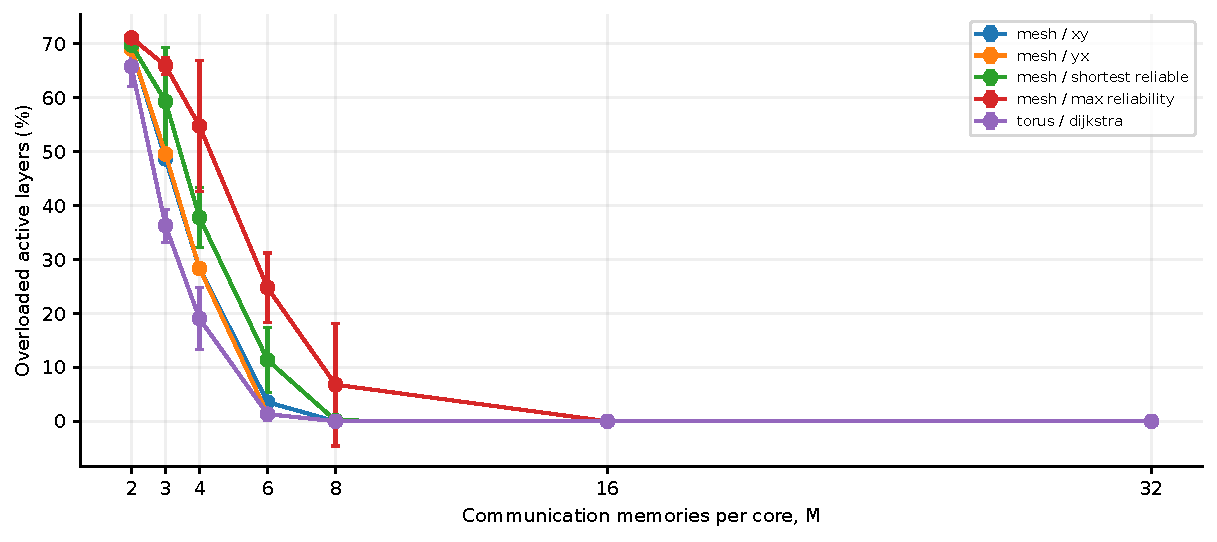
\includegraphics[width=.94\linewidth,height=.34\textheight,keepaspectratio]{figures/summary/congestion_route_overloaded_layer_percent.pdf}\captionof{figure}{Mean and sample SD across three conceptual reliability-seed labels. Identical route aliases are not independent mappings.}\end{center}
\begin{center}{\scriptsize\setlength{\tabcolsep}{3pt}
\begin{tabular}{lrrrrr}
\toprule
M & XY & YX & Short-rel & Max-rel & Torus Dijk. \\
\midrule
2 & $69.027\pm0.000$ & $69.027\pm0.000$ & $69.764\pm1.842$ & $71.091\pm0.255$ & $65.782\pm3.763$ \\
3 & $48.673\pm0.000$ & $49.558\pm0.000$ & $59.292\pm10.051$ & $65.929\pm1.595$ & $36.283\pm3.066$ \\
4 & $28.319\pm0.000$ & $28.319\pm0.000$ & $37.758\pm5.568$ & $54.720\pm12.137$ & $19.027\pm5.752$ \\
6 & $3.540\pm0.000$ & $1.327\pm0.000$ & $11.357\pm6.104$ & $24.779\pm6.427$ & $1.327\pm1.171$ \\
8 & $0.0000\pm0.0000$ & $0.0000\pm0.0000$ & $0.1475\pm0.2555$ & $6.785\pm11.370$ & $0.0000\pm0.0000$ \\
16 & $0.0000\pm0.0000$ & $0.0000\pm0.0000$ & $0.0000\pm0.0000$ & $0.0000\pm0.0000$ & $0.0000\pm0.0000$ \\
32 & $0.0000\pm0.0000$ & $0.0000\pm0.0000$ & $0.0000\pm0.0000$ & $0.0000\pm0.0000$ & $0.0000\pm0.0000$ \\
\bottomrule\end{tabular}}
\captionof{table}{Overloaded active layers (\%) for route counting.}
{\footnotesize\href{https://github.com/sanjeevkrishnaa/Compiler-Driven-ACE/blob/codex/ace-scheduler-correctness/docs/latex/qft96_final/data/congestion_overview.csv}{Exact CSV values and sample counts}}
\end{center}
\clearpage\section*{Route counting: Overloaded core-layers}
\begin{center}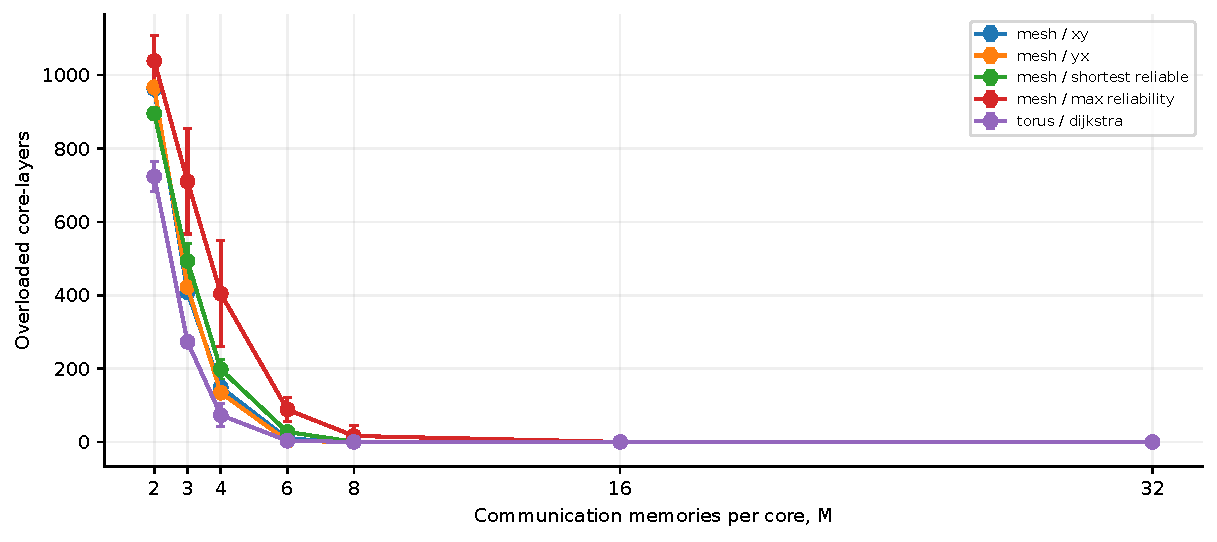
\includegraphics[width=.94\linewidth,height=.34\textheight,keepaspectratio]{figures/summary/congestion_route_overloaded_core_layers.pdf}\captionof{figure}{Mean and sample SD across three conceptual reliability-seed labels. Identical route aliases are not independent mappings.}\end{center}
\begin{center}{\scriptsize\setlength{\tabcolsep}{3pt}
\begin{tabular}{lrrrrr}
\toprule
M & XY & YX & Short-rel & Max-rel & Torus Dijk. \\
\midrule
2 & $962.00\pm0.00$ & $967.00\pm0.00$ & $895.33\pm15.04$ & $1038.67\pm70.49$ & $723.67\pm41.96$ \\
3 & $408.00\pm0.00$ & $422.00\pm0.00$ & $493.33\pm47.35$ & $710.33\pm143.49$ & $273.00\pm4.36$ \\
4 & $149.00\pm0.00$ & $134.00\pm0.00$ & $197.67\pm27.75$ & $404.33\pm144.07$ & $73.000\pm31.048$ \\
6 & $9.000\pm0.000$ & $3.000\pm0.000$ & $27.333\pm13.429$ & $88.333\pm33.292$ & $3.333\pm2.887$ \\
8 & $0.0000\pm0.0000$ & $0.0000\pm0.0000$ & $0.3333\pm0.5774$ & $16.333\pm27.429$ & $0.0000\pm0.0000$ \\
16 & $0.0000\pm0.0000$ & $0.0000\pm0.0000$ & $0.0000\pm0.0000$ & $0.0000\pm0.0000$ & $0.0000\pm0.0000$ \\
32 & $0.0000\pm0.0000$ & $0.0000\pm0.0000$ & $0.0000\pm0.0000$ & $0.0000\pm0.0000$ & $0.0000\pm0.0000$ \\
\bottomrule\end{tabular}}
\captionof{table}{Overloaded core-layers for route counting.}
{\footnotesize\href{https://github.com/sanjeevkrishnaa/Compiler-Driven-ACE/blob/codex/ace-scheduler-correctness/docs/latex/qft96_final/data/congestion_overview.csv}{Exact CSV values and sample counts}}
\end{center}
\clearpage\section*{Route counting: Excess demand}
\begin{center}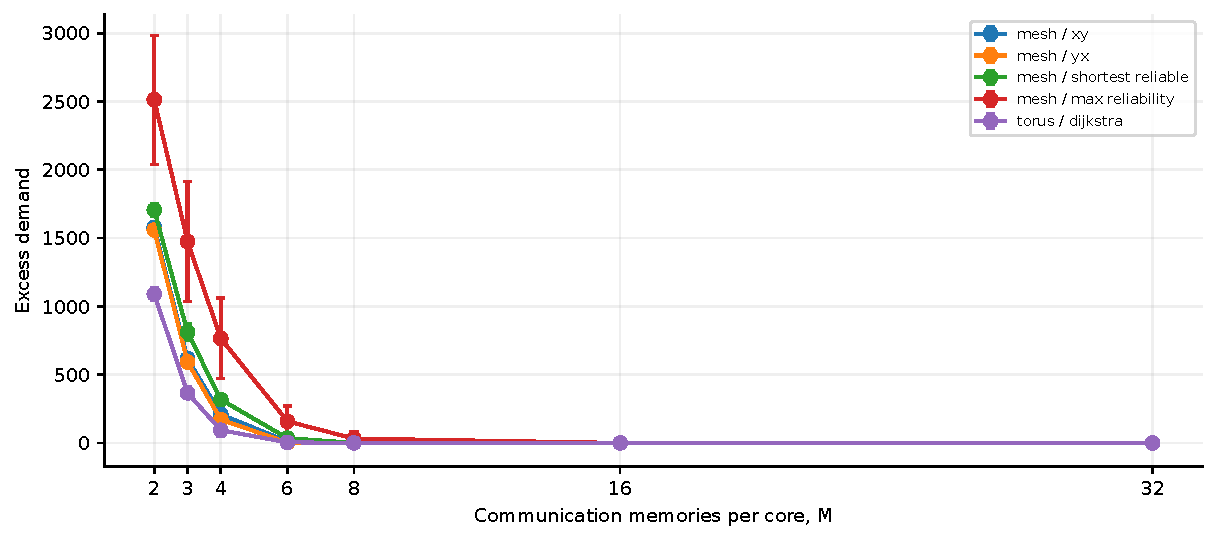
\includegraphics[width=.94\linewidth,height=.34\textheight,keepaspectratio]{figures/summary/congestion_route_excess_demand.pdf}\captionof{figure}{Mean and sample SD across three conceptual reliability-seed labels. Identical route aliases are not independent mappings.}\end{center}
\begin{center}{\scriptsize\setlength{\tabcolsep}{3pt}
\begin{tabular}{lrrrrr}
\toprule
M & XY & YX & Short-rel & Max-rel & Torus Dijk. \\
\midrule
2 & $1579.00\pm0.00$ & $1560.00\pm0.00$ & $1706.33\pm47.65$ & $2514.00\pm472.90$ & $1090.00\pm50.21$ \\
3 & $617.00\pm0.00$ & $593.00\pm0.00$ & $811.00\pm62.22$ & $1475.33\pm438.79$ & $366.33\pm43.39$ \\
4 & $209.00\pm0.00$ & $171.00\pm0.00$ & $317.67\pm17.62$ & $765.00\pm296.14$ & $93.333\pm46.608$ \\
6 & $11.000\pm0.000$ & $3.000\pm0.000$ & $35.000\pm17.349$ & $158.33\pm112.17$ & $4.667\pm4.163$ \\
8 & $0.0000\pm0.0000$ & $0.0000\pm0.0000$ & $0.3333\pm0.5774$ & $32.000\pm54.562$ & $0.0000\pm0.0000$ \\
16 & $0.0000\pm0.0000$ & $0.0000\pm0.0000$ & $0.0000\pm0.0000$ & $0.0000\pm0.0000$ & $0.0000\pm0.0000$ \\
32 & $0.0000\pm0.0000$ & $0.0000\pm0.0000$ & $0.0000\pm0.0000$ & $0.0000\pm0.0000$ & $0.0000\pm0.0000$ \\
\bottomrule\end{tabular}}
\captionof{table}{Excess demand for route counting.}
{\footnotesize\href{https://github.com/sanjeevkrishnaa/Compiler-Driven-ACE/blob/codex/ace-scheduler-correctness/docs/latex/qft96_final/data/congestion_overview.csv}{Exact CSV values and sample counts}}
\end{center}
\clearpage\section*{Hop counting: Overloaded active layers (\%)}
\begin{center}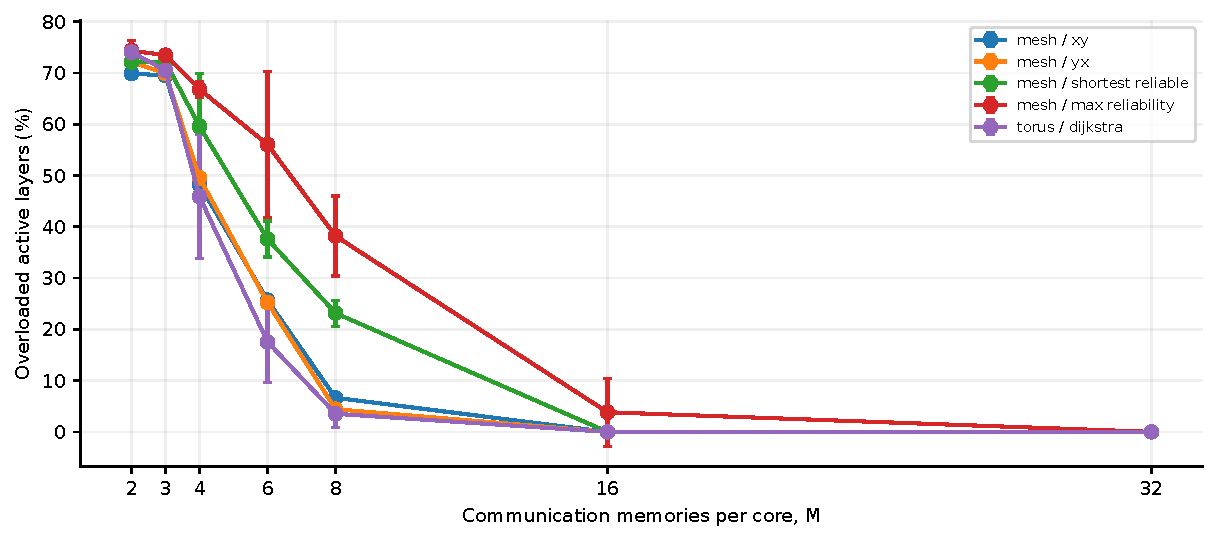
\includegraphics[width=.94\linewidth,height=.34\textheight,keepaspectratio]{figures/summary/congestion_hop_overloaded_layer_percent.pdf}\captionof{figure}{Mean and sample SD across three conceptual reliability-seed labels. Identical route aliases are not independent mappings.}\end{center}
\begin{center}{\scriptsize\setlength{\tabcolsep}{3pt}
\begin{tabular}{lrrrrr}
\toprule
M & XY & YX & Short-rel & Max-rel & Torus Dijk. \\
\midrule
2 & $69.912\pm0.000$ & $72.124\pm0.000$ & $72.124\pm1.533$ & $74.336\pm1.929$ & $74.041\pm0.921$ \\
3 & $69.469\pm0.000$ & $69.912\pm0.000$ & $72.124\pm1.533$ & $73.451\pm0.442$ & $70.501\pm1.114$ \\
4 & $48.230\pm0.000$ & $49.558\pm0.000$ & $59.587\pm10.257$ & $66.814\pm1.595$ & $45.870\pm12.120$ \\
6 & $25.664\pm0.000$ & $25.221\pm0.000$ & $37.611\pm3.512$ & $56.047\pm14.299$ & $17.552\pm7.919$ \\
8 & $6.637\pm0.000$ & $4.425\pm0.000$ & $23.156\pm2.516$ & $38.201\pm7.795$ & $3.540\pm2.763$ \\
16 & $0.0000\pm0.0000$ & $0.0000\pm0.0000$ & $0.0000\pm0.0000$ & $3.835\pm6.642$ & $0.0000\pm0.0000$ \\
32 & $0.0000\pm0.0000$ & $0.0000\pm0.0000$ & $0.0000\pm0.0000$ & $0.0000\pm0.0000$ & $0.0000\pm0.0000$ \\
\bottomrule\end{tabular}}
\captionof{table}{Overloaded active layers (\%) for hop counting.}
{\footnotesize\href{https://github.com/sanjeevkrishnaa/Compiler-Driven-ACE/blob/codex/ace-scheduler-correctness/docs/latex/qft96_final/data/congestion_overview.csv}{Exact CSV values and sample counts}}
\end{center}
\clearpage\section*{Hop counting: Overloaded core-layers}
\begin{center}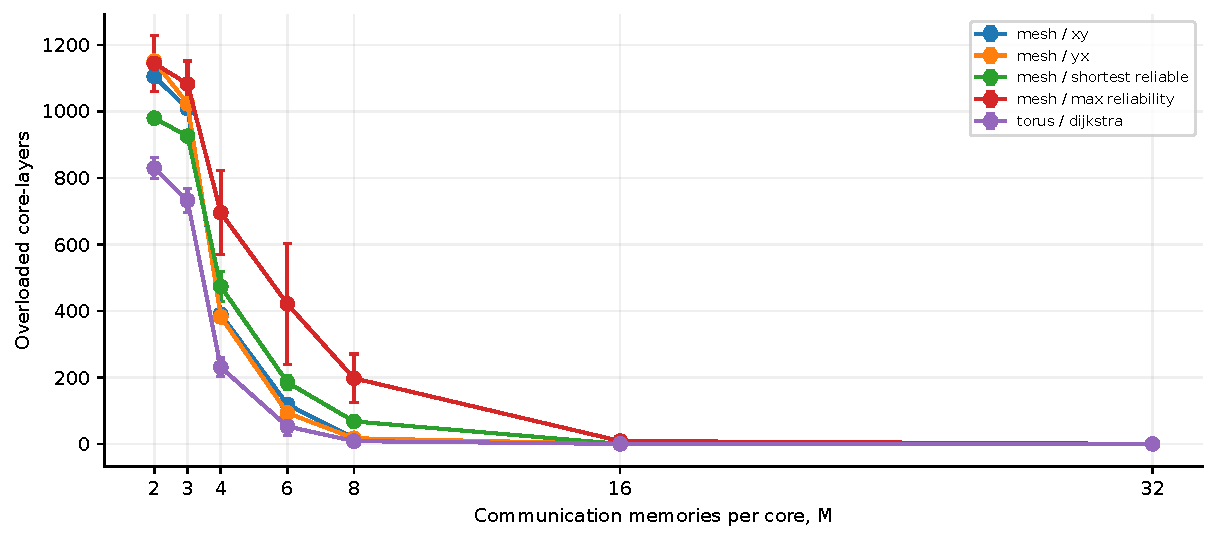
\includegraphics[width=.94\linewidth,height=.34\textheight,keepaspectratio]{figures/summary/congestion_hop_overloaded_core_layers.pdf}\captionof{figure}{Mean and sample SD across three conceptual reliability-seed labels. Identical route aliases are not independent mappings.}\end{center}
\begin{center}{\scriptsize\setlength{\tabcolsep}{3pt}
\begin{tabular}{lrrrrr}
\toprule
M & XY & YX & Short-rel & Max-rel & Torus Dijk. \\
\midrule
2 & $1105.00\pm0.00$ & $1151.00\pm0.00$ & $979.67\pm15.01$ & $1144.33\pm85.15$ & $829.33\pm31.77$ \\
3 & $1008.00\pm0.00$ & $1023.00\pm0.00$ & $925.67\pm10.02$ & $1082.67\pm68.81$ & $731.67\pm36.47$ \\
4 & $390.00\pm0.00$ & $382.00\pm0.00$ & $473.33\pm45.94$ & $695.33\pm126.77$ & $230.33\pm28.01$ \\
6 & $119.00\pm0.00$ & $93.000\pm0.000$ & $185.00\pm21.52$ & $420.67\pm181.48$ & $52.667\pm28.361$ \\
8 & $17.000\pm0.000$ & $17.000\pm0.000$ & $67.667\pm9.238$ & $197.33\pm73.11$ & $8.333\pm6.429$ \\
16 & $0.0000\pm0.0000$ & $0.0000\pm0.0000$ & $0.0000\pm0.0000$ & $8.667\pm15.011$ & $0.0000\pm0.0000$ \\
32 & $0.0000\pm0.0000$ & $0.0000\pm0.0000$ & $0.0000\pm0.0000$ & $0.0000\pm0.0000$ & $0.0000\pm0.0000$ \\
\bottomrule\end{tabular}}
\captionof{table}{Overloaded core-layers for hop counting.}
{\footnotesize\href{https://github.com/sanjeevkrishnaa/Compiler-Driven-ACE/blob/codex/ace-scheduler-correctness/docs/latex/qft96_final/data/congestion_overview.csv}{Exact CSV values and sample counts}}
\end{center}
\clearpage\section*{Hop counting: Excess demand}
\begin{center}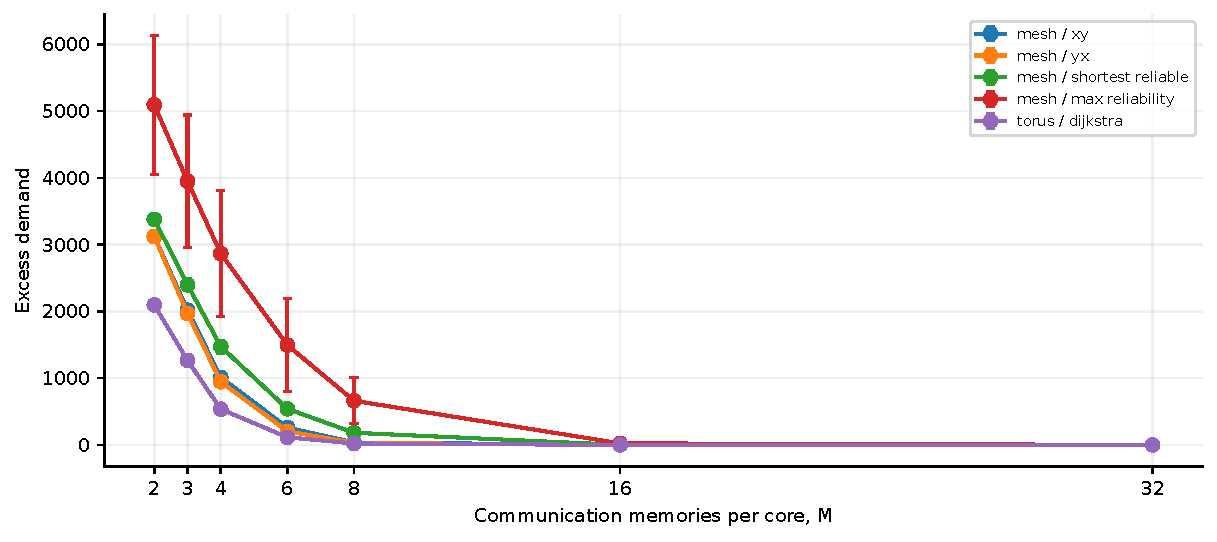
\includegraphics[width=.94\linewidth,height=.34\textheight,keepaspectratio]{figures/summary/congestion_hop_excess_demand.pdf}\captionof{figure}{Mean and sample SD across three conceptual reliability-seed labels. Identical route aliases are not independent mappings.}\end{center}
\begin{center}{\scriptsize\setlength{\tabcolsep}{3pt}
\begin{tabular}{lrrrrr}
\toprule
M & XY & YX & Short-rel & Max-rel & Torus Dijk. \\
\midrule
2 & $3124.00\pm0.00$ & $3120.00\pm0.00$ & $3378.00\pm77.95$ & $5093.33\pm1045.34$ & $2096.33\pm48.79$ \\
3 & $2019.00\pm0.00$ & $1969.00\pm0.00$ & $2398.33\pm89.20$ & $3949.00\pm992.16$ & $1267.00\pm42.23$ \\
4 & $1011.00\pm0.00$ & $946.00\pm0.00$ & $1472.67\pm97.39$ & $2866.33\pm946.75$ & $535.33\pm52.79$ \\
6 & $260.00\pm0.00$ & $203.00\pm0.00$ & $540.33\pm24.21$ & $1495.00\pm691.03$ & $114.00\pm72.19$ \\
8 & $36.000\pm0.000$ & $30.000\pm0.000$ & $181.67\pm49.07$ & $661.33\pm341.95$ & $21.667\pm18.230$ \\
16 & $0.0000\pm0.0000$ & $0.0000\pm0.0000$ & $0.0000\pm0.0000$ & $23.000\pm39.837$ & $0.0000\pm0.0000$ \\
32 & $0.0000\pm0.0000$ & $0.0000\pm0.0000$ & $0.0000\pm0.0000$ & $0.0000\pm0.0000$ & $0.0000\pm0.0000$ \\
\bottomrule\end{tabular}}
\captionof{table}{Excess demand for hop counting.}
{\footnotesize\href{https://github.com/sanjeevkrishnaa/Compiler-Driven-ACE/blob/codex/ace-scheduler-correctness/docs/latex/qft96_final/data/congestion_overview.csv}{Exact CSV values and sample counts}}
\end{center}